\begin{figure*}[t]
  \centering
  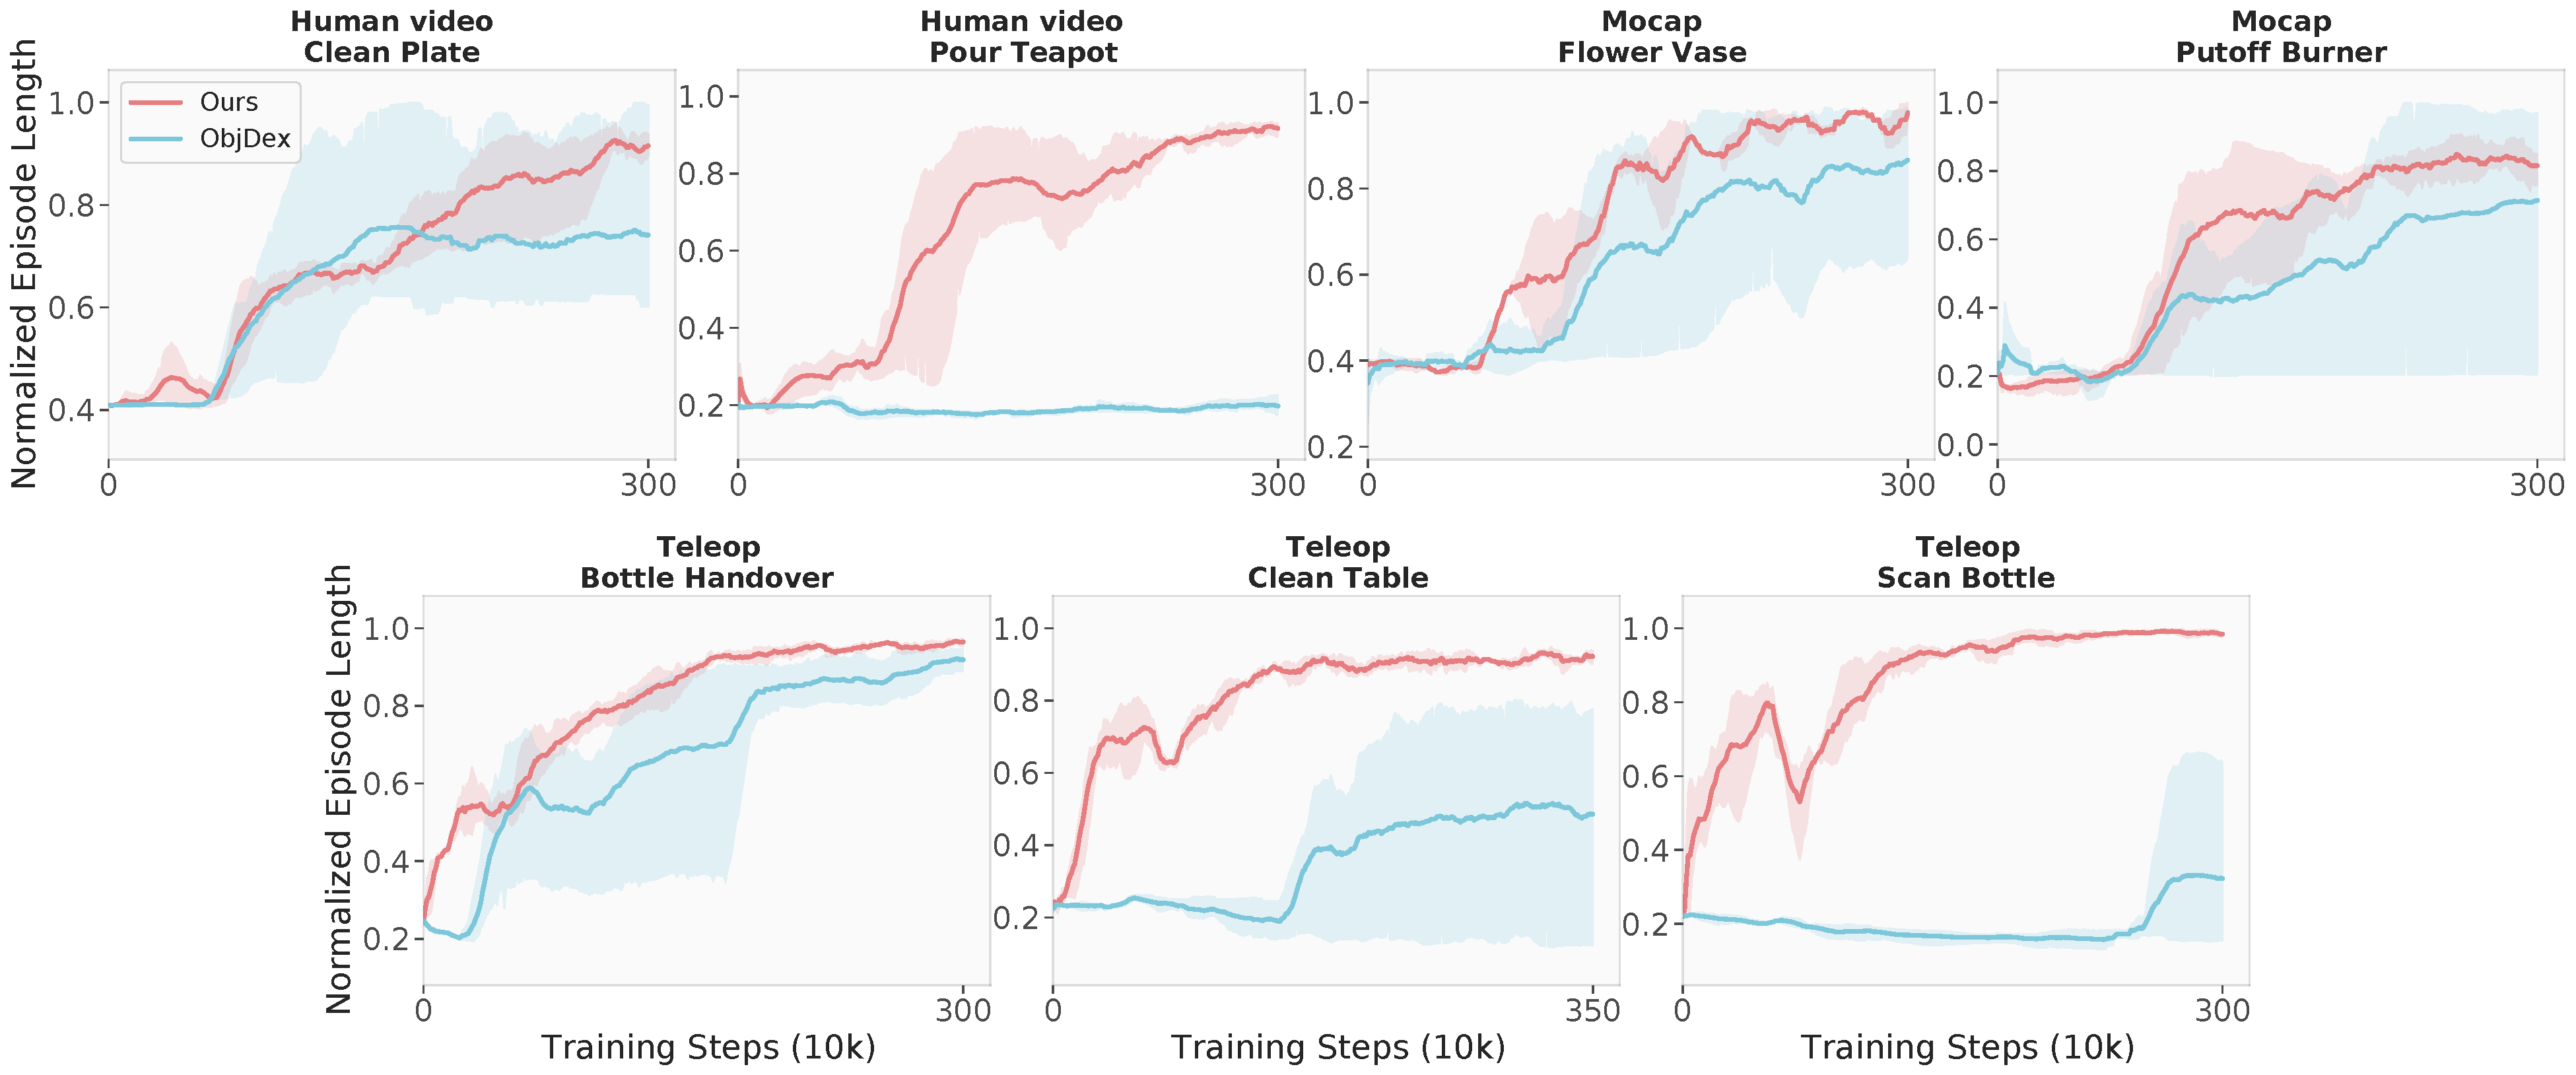
\includegraphics[width=1.0\linewidth]{figures/train_curve_new.pdf}
  \caption{ \textbf{The training curve of \ourshort.} The horizontal axis denotes the training steps, while the vertical axis represents the normalized task length successfully accomplished by the policy. \textit{Teleop} refers to one-shot human motion teleoperation in simulation, \textit{Human video} denotes trajectories extracted from video data, and \textit{Mocap} corresponds to motion derived from mocap datasets. \ourshort not only demonstrates the capability to accomplish diverse manipulation tasks originating from various forms of human motion, but also exhibits superior sample efficiency throughout training. All results are evaluated across 3 seeds. }
  \label{fig:train_curve}
\end{figure*}